\section{Introduction}
% problem description: semantic relatedness
Computing semantic relatedness(SR) between two elements(words, sentences,
texts etc.) is a fundamental task for many applications in Natural Language
Processing(NLP) such as lexicon induction(\cite{aaai/QadirMGL15}), Named 
Entity Disambiguation{\cite{acl/HanZ10}}, Keyword Extraction
(\cite{ijcai/ZhangFW13}) and Information Retrieval(\cite{acl/GurevychMZ07}). 
Additionaly, computing semantic relatedness contributes other applications, 
for example, opinion spam problem (\cite{www/SandulescuE15}) and so on(+some example). 
In this paper we focus on computing semantic relatedness between two 
words in knowledge graph with neural network.

It has long been thought that when human measure the relatedness between
a pair of words, a deeper reasoning is triggered to compare the concepts
behind the words. Many traditional studies on semantic relatedness
utilize different data sources. There are
i) \emph{the large corpora}, such as wikipedia(\cite{ijcai/GabrilovichM07}), 
ii) \emph{the lexical databases}, such as WordNet(\cite{acl/Pucher07}) or Wikithionary(\cite{aaai/ZeschMG08}), 
iii) \emph{the knowledge graph}, such as DBpedia(\cite{aaai/NavigliP12}) or BabelNet(\cite{aaai/NavigliP12}).
With the development knowledge representation, computing semantic relatedness utilizing
knowledge-rich resouce is a well-explored line of research. It is known to us all that
knowledge graph contains both syntactic and semantic information which are 
richer than lexical databases, and more sturctured knowledge than the large corpora.
On the account of advantages of knowledge graph, we utilize it as background 
knowledge to compute semantic relatedness.

% Knowledge graph can be accessed with powerful query language Sparql in RDF graph.
% As for the methods build on the data soruce, the recent word embedding 
% learning approaches demonstrate their abilities
% to capture syntactic and semantic information, and outperform the
% lexicon-based methods\cite{acl/Pucher07}. 
% Knowledge Graph, as a semantic graph, stores
% vast amount of sturctured knowledge. 

\begin{figure*}
    \centering
    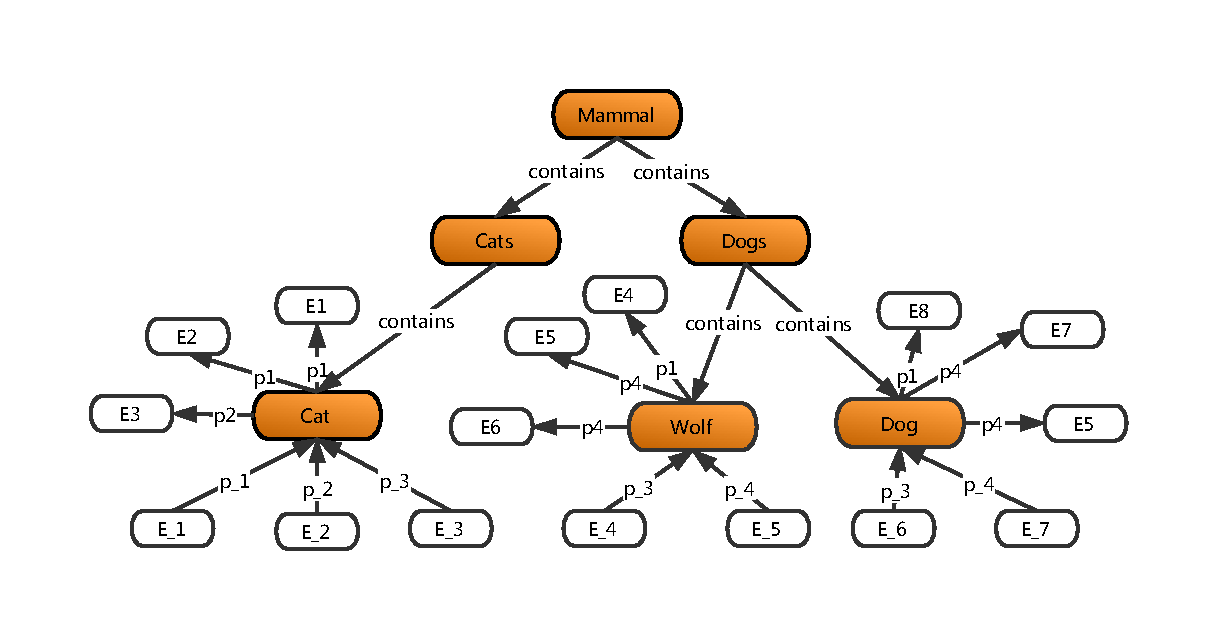
\includegraphics[width=1.0\textwidth]{pic/introduction.pdf}\\
    \caption{Subgraph example in knowledge graph}
    \label{weak1}
\end{figure*}

Recently, there are some researchs having attached importance to measure semantic relatedness
in knowledge graph\cite{aaai/Pirro12, aaai/NavigliP12, acl/IacobacciPN15}. 
\cite{acl/IacobacciPN15} leverage entity linking to annotate the dump of wikipedia. Based on this,
the sense-annotated corpus is generated. Then the author use word2vec to
train the sense-annotated corpus getting distributed representation of different 
word senses. This step still need a significant preprocessing and data transformation efforts. 
As we can see this approach computing semantic relatedness on account of large corpora.
The author just put the knowledge graph on the position of support. 
\cite{aaai/NavigliP12} presents a knowledge-rich approach to computing multilingual semantic
relatedness which exploits the joint contribution of different languages. Given a pair of words 
in two languages they use BabelNet to collect their translations, compute semantic
graphs in a variety of languages, and then combine the empirical evidence from these 
different languages by intersecting their respective graphs.
\cite{aaai/Pirro12} propose an approach exploiting the graph nature of RDF and SPARQL query
Language to access knowledge graph. It not only obtains the comparable
result with the state-of-art model at that moment, but also avoids the burden
of preprocessing and data transformation.

Though \cite{aaai/Pirro12} avoids a significant preprocessing and data
transformation effort, develops scalability of their approach while adopting 
the knowledge graph. However, they miss some factors which
might contribute to semantic relatedness measurement. Firstly, given two words
as input, the first step is to find corresponding entities in knowledge
graph. Obviously, there are usually more than one corresponding entity for a single word.
For an input word \emph{car}, for example, we will get \emph{:Automobile} and
\emph{:Auto\underline{\hspace{0.5em}}Racing} and so on. \cite{aaai/Pirro12} lose
sight of the informativeness of the other entities, while they just
consider the entity with the highest rank. Secondly, \cite{aaai/Pirro12} misses
some informativeness of \emph{objects} in \emph{triple(subject, prediacte, object)} as their strategy takes
the predicates into account exclusively based on the TFIDF. This
method ignored the function of \emph{objects} in a semantic triple.

As show in Fig\ref{weak1}, subgraph contains \emph{Dogs} and \emph{Cats} extracted from
knowledge. We simplify the sepcific features of entities to concise symbol. 
We can see that entities in knowledge graph such as \emph{Cat} plays the role 
of both \emph{Object(Cats contains Cat)} and \emph{Subject(Cat $p_1$ $E_1$)}
in a pattern of triple. The predicate which is connected with a entity(Cat)
may be regarded as an outgoing($p_1$) or incoming predicate($p_{_1}$).
In \cite{aaai/Pirro12}, the relatedness space for a entity ${E_i}$ is modelled a 
k-dimensional weighted vector \emph{V$_i$}, where each dimension represents
the informativeness of a specific predicate.
For example, the weighted vector for \emph{Cat} is 
$[v_{p_1}^o, v_{p_2}^o, v_{p_\_1}^i, v_{p_\_2}^i, v_{p_\_2}^i]$ in which $v_{p_i}^o$ 
means the vector value of outgoing predicate $p_i$ and $v_{p_j}^i$ 
means the vector value of incoming predicate $p_j$. 
In this example, for the specific \emph{predicate} $p_1$, there are two triples:
\emph{(Cat $p_1$ $E_1$)} and \emph{(Cat $p_2$ $E_2$)} describe the entity \emph{Cat}.
The way of \cite{aaai/Pirro12} in which they get the contribute of $p_i$ is the number
of triples of the form \emph{(Cat $p_1$ ?)} where the $p_1$ as a outgoing predicate
divided by the total number of triples in which \emph{Cat} appears
((Cat $p_1$ $E_1$), (Cat $p_1$ $E_2$), (Cat $p_2$ $E_3$)), i.e., $v_{p_1}^o$=2/3.
They just ignore the function of a set of specific objects in a pattern of triple.
Besides, there is another aspect they have ignored. In this example, for entities $Cat$,
$Dog$ and $Wolf$, let us see the informativeness of prediacte $p_1$. We get
\emph{{(Cat $p_1$ $E_1$),(Cat $p_1$ $E_2$),(Cat $p_1$ $E_4$),(Cat $p_1$ $E_8$)}}. 
It is obvious that when they compute relatedness between \emph{Cat} and \emph{Wolf}, they get the
vector value in outgoing predicate $p_1$ of \emph{Wolf} as same as the \emph{Dog}.
In other words in the compare of dimension of predicate $p_1$ between \emph{Cat} and \emph{Wolf},
\emph{Cat} and \emph{Dog}, they get no difference. Obviously, the author do not distinguish the different 
objects w.r.t a specific predicate. In order to improve the perfomance of the computing
semantic relatedness based on knowledge graph, we propose a model to touch 
the target. Our model is shown as below:

1. For given word pairs, the first job is to query the corresponding entities. In order to use the
neural network for training the dataset, we also need to construct a graph contains all related
entities, attributes and relations between the corresponding entity pairs.

2. We use Starspace proposed by Facebook for knowledge graph instead of Word2vec to train the subgraph
extracted from the knowledge graph. Then we can get a distributional representation(vector) for each
entities and predicates. 

3. When we take as inputs a word, we can get several corresponding entities.
Inspired by \cite{acl/IacobacciPN15}, we utilize a approach to combine the 
relatedness scores gathering from the compare of entity paris
as the finnal semantic relatedness score in knowledge graph.

This paper is organized as below. 